\documentclass{article}
\usepackage{color}
\usepackage{graphicx}
\usepackage{multirow}
\usepackage{float}
\usepackage{amsmath,amsfonts,amsthm,amssymb}
\usepackage{geometry}
\usepackage{enumerate}
\usepackage{fancyhdr}
\usepackage{subfigure}
\usepackage{listings}
\pagestyle{fancyplain}
\lhead{VE311\\Assignment1}
\rhead{Zhang Tianchi\\516370910233}
\cfoot{\thepage}
\begin{document}
\section*{Q1}
\begin{enumerate}[(a)]
	\item 
	\begin{align*}
	e^{q\Phi_n/(kT)}&=10^{19-(10-(10-17))}=10^{16}\\
	\Phi_i &= 16\ln(10)\frac{kT}{q}=0.9533\ V\\\\
	x_d &= [\frac{2\epsilon_{Si}}{q}\Phi_i(1/N_a+1/N_d) ]^{0.5}=0.1116\ \mu m\\
	x_p &= \frac{N_d}{N_a+N_d}=0.1105\ \mu m\\
	x_n &= \frac{N_a}{N_a+N_d}=0.0011\ \mu m\\\\
	E_{max} &=\frac{-qN_ax_p}{\epsilon_{Si}}=-1.715\times 10^5\ V/cm
	\end{align*}
	\item 
	When $V_a = 1\ V$
	$$C_j=\frac{A\epsilon_{Si}}{x_d}\frac{1}{\sqrt{1+\frac{V_a}{\Phi_i}}}=3.241\times 10^{-12}\ F$$
	When $V_a = 10\ V$
	$$C_j=\frac{A\epsilon_{Si}}{x_d}\frac{1}{\sqrt{1+\frac{V_a}{\Phi_i}}}=1.369\times 10^{-12}\ F$$
	The capacitance decrease when the reverse bias increases. $C_j\times\sqrt{V_a}$ changed little when they change.
	\item 
	\begin{align*}
	\mu_p &= 150cm^2/(Vs)\qquad D_p=\frac{kT}{q}\mu_p=3.881\ cm^2/s\\
	\mu_n &= 750cm^2/(Vs)\qquad D_p=\frac{kT}{q}\mu_p=19.401\ cm^2/s\\
	L_p&=3.5\mu m\qquad L_n=75\ \mu m\\
	I_p&=qAn_i^2(\frac{D_p}{L_pN_d}+\frac{D_n}{L_nN_a})(e^\frac{-qV_a}{kT}-1)=1.3134\ A
	\end{align*}
\end{enumerate}
\newpage
\section*{Q2}
\begin{enumerate}[(a)]
	\item 
	$$I_D=I_S(e^\frac{q(V_in-V_out)}{kT}-1)$$
	When $V_{in}-V_{out}\rightarrow0$, $i.e.$ $\frac{q(V_in-V_out)}{kT}\rightarrow0$,we have
	$$e^\frac{q(V_in-V_out)}{kT}\rightarrow1+\frac{q(V_in-V_out)}{kT}$$
	so $I_D\rightarrow I_S\times \frac{q(V_in-V_out)}{kT}$ when $V_{in}-V_{out}\rightarrow0$, $i.e.$ their relationship is Linear.\\\\	
	Code: 
	\begin{lstlisting}
	Voltage Divider - DC
	.model Dbreak D Is=1e-16 Rs=0 N=1 TT=0 Cjo=0pF
	.DC vin -2 2 0.01
	vin 1 0
	d1 1 2 Dbreak
	r1 2 0 1.0k
	.end
	\end{lstlisting}
	Graph: 
	\begin{figure}[H]
		\centering 
		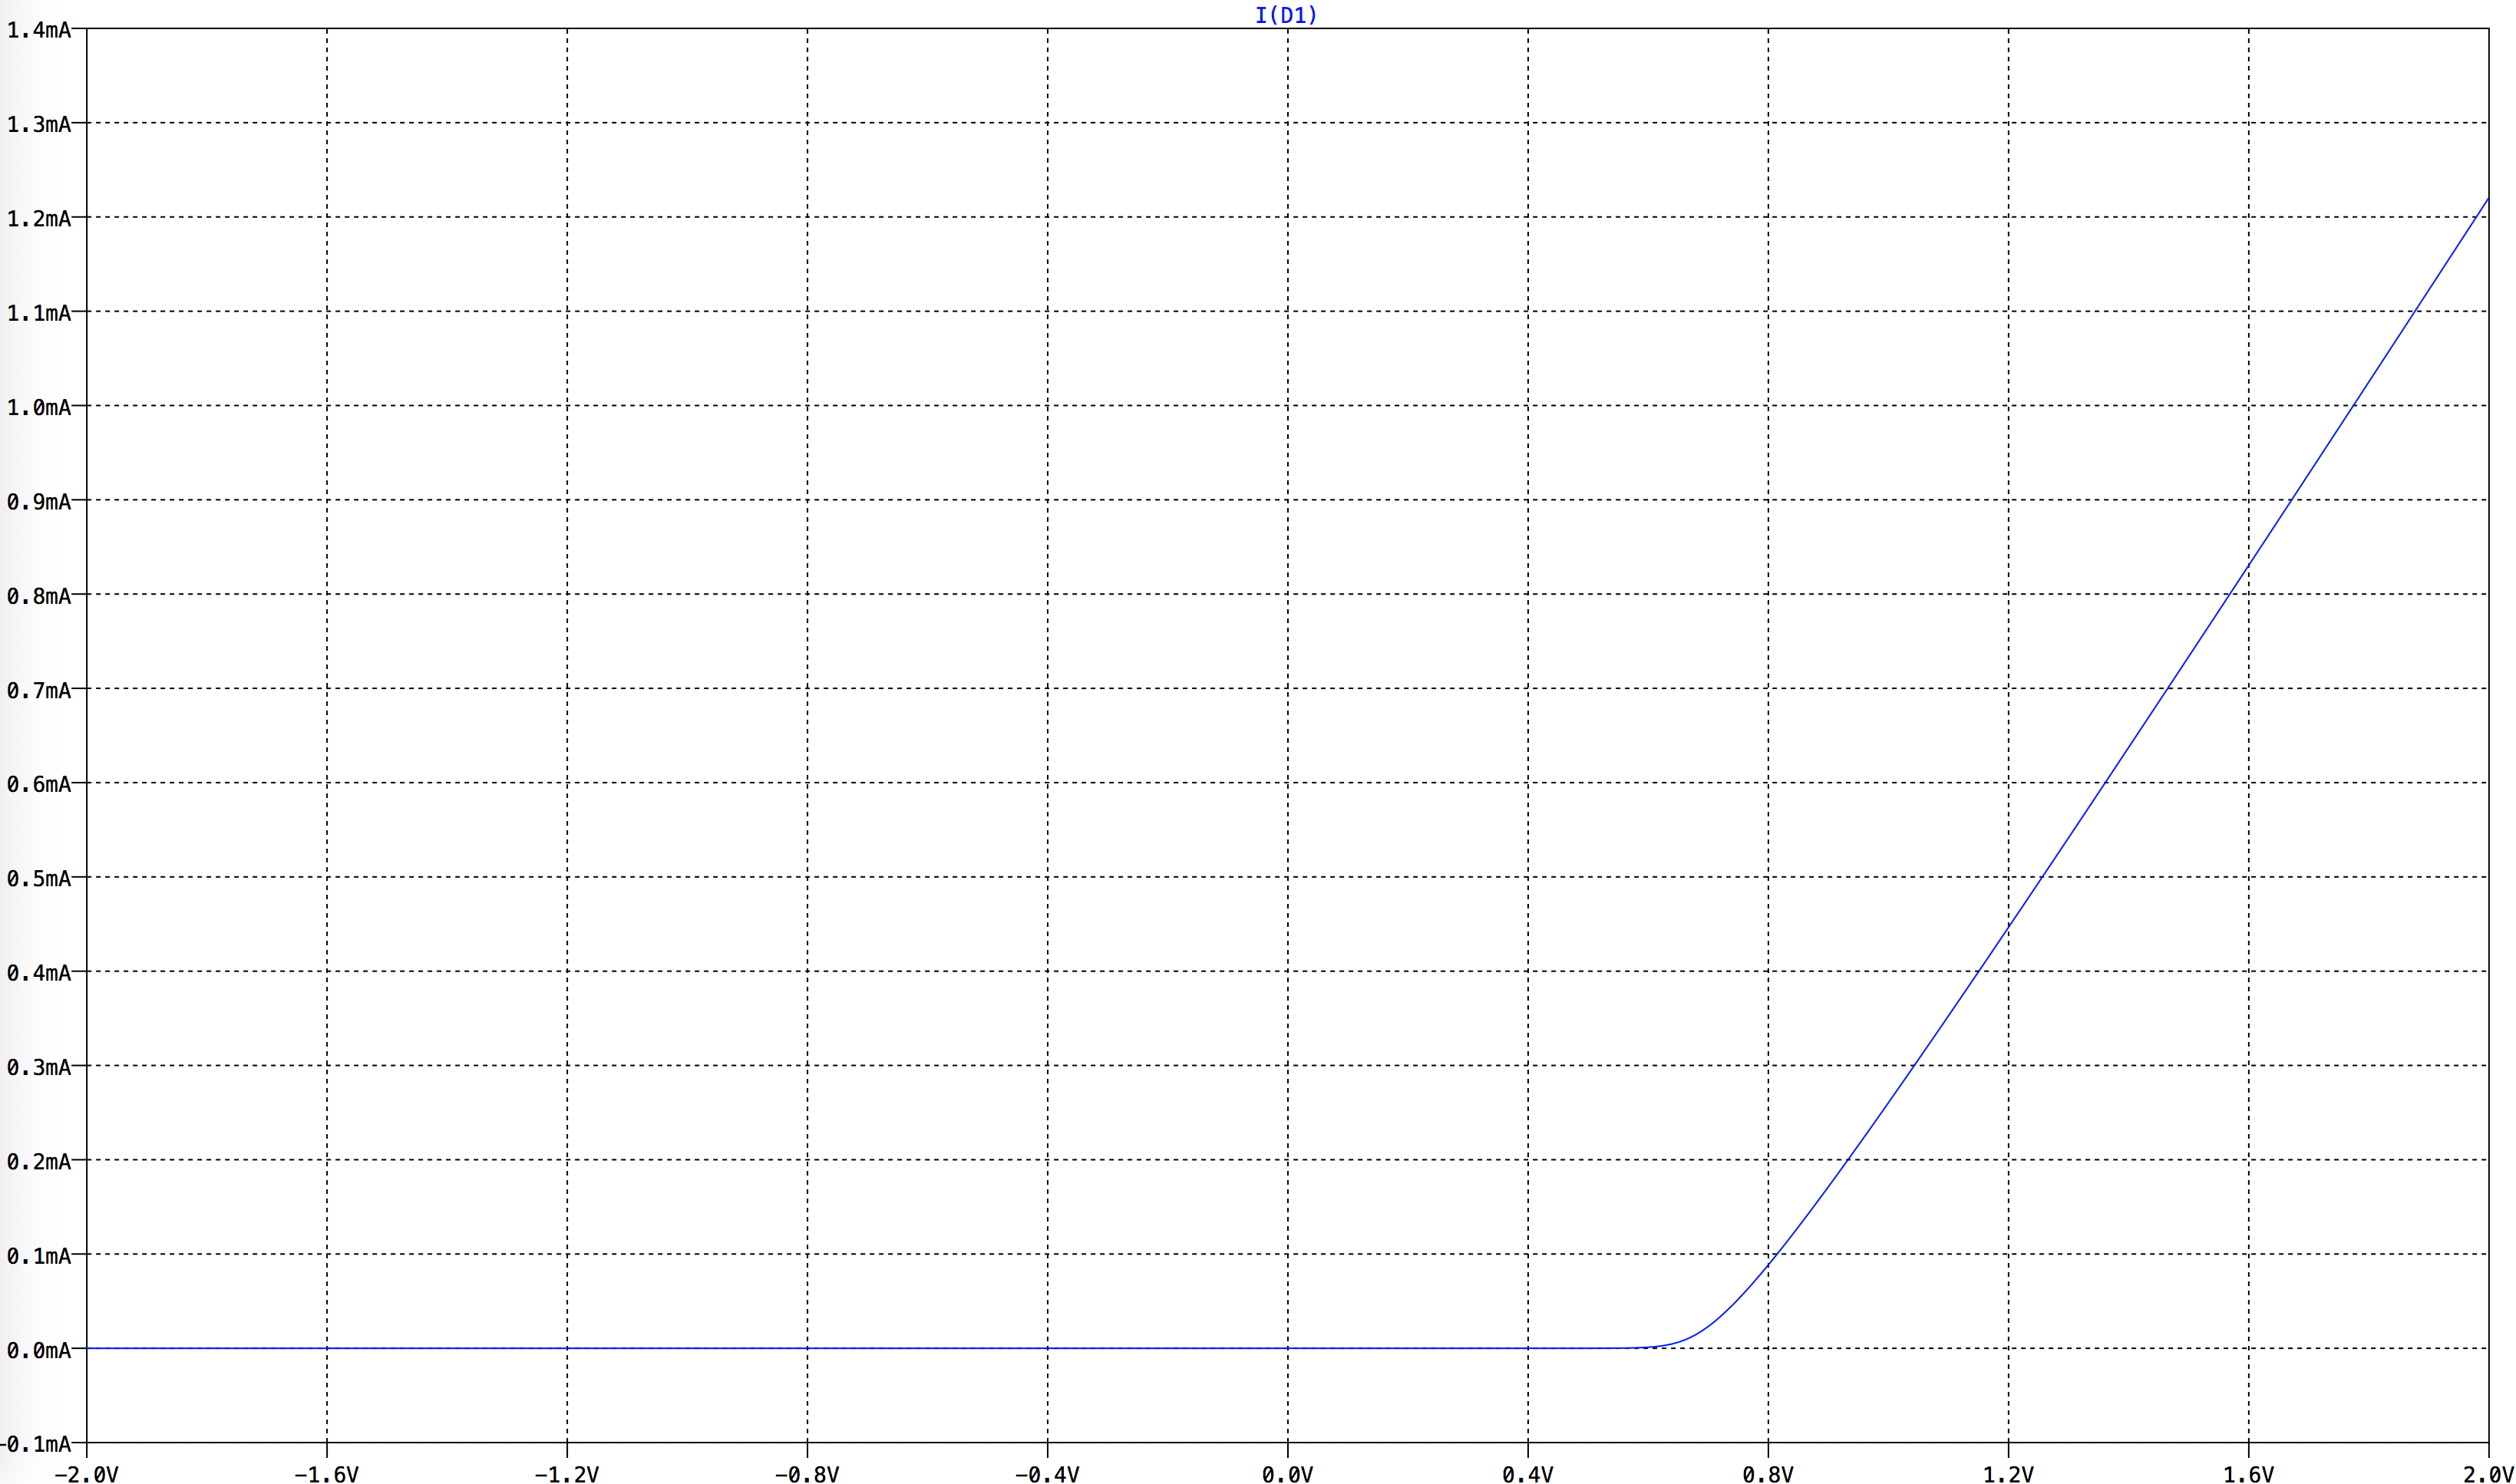
\includegraphics [width=0.8\linewidth]{2_a.png}
		\caption{2\_b}
	\end{figure}
\newpage
	\item 
	According to property of diode, $V_out\geq0$. And we have $V_{out} + V_D = V_{in}$. In the first half period, when $V_{in}$ is small, $V_D$ is much larger than $V_{out}$, so there is a "delay" of increase. When $V_{in}$ is large enough, $V_{in}$ and $V_{out}$ behave similarly. In the second half period, $V_{in} <0$ but $V_out\geq0$, so $V_{out}=0$.\\\\
	Code: 
	\begin{lstlisting}
	Voltage Divider - Sine
	.model Dbreak D Is=1e-16 Rs=0 N=1 TT=0 Cjo=0pF
	vin 1 0 sin (0.0V 2.0V 60) ac 1.0 dc 0.0
	d1 1 2 Dbreak
	r1 2 0 1.0k
	.control
	tran 0.1ms 30ms
	plot v(1) v(2)
	.end
	\end{lstlisting}
	Graph: 
	\begin{figure}[H]
		\centering 
		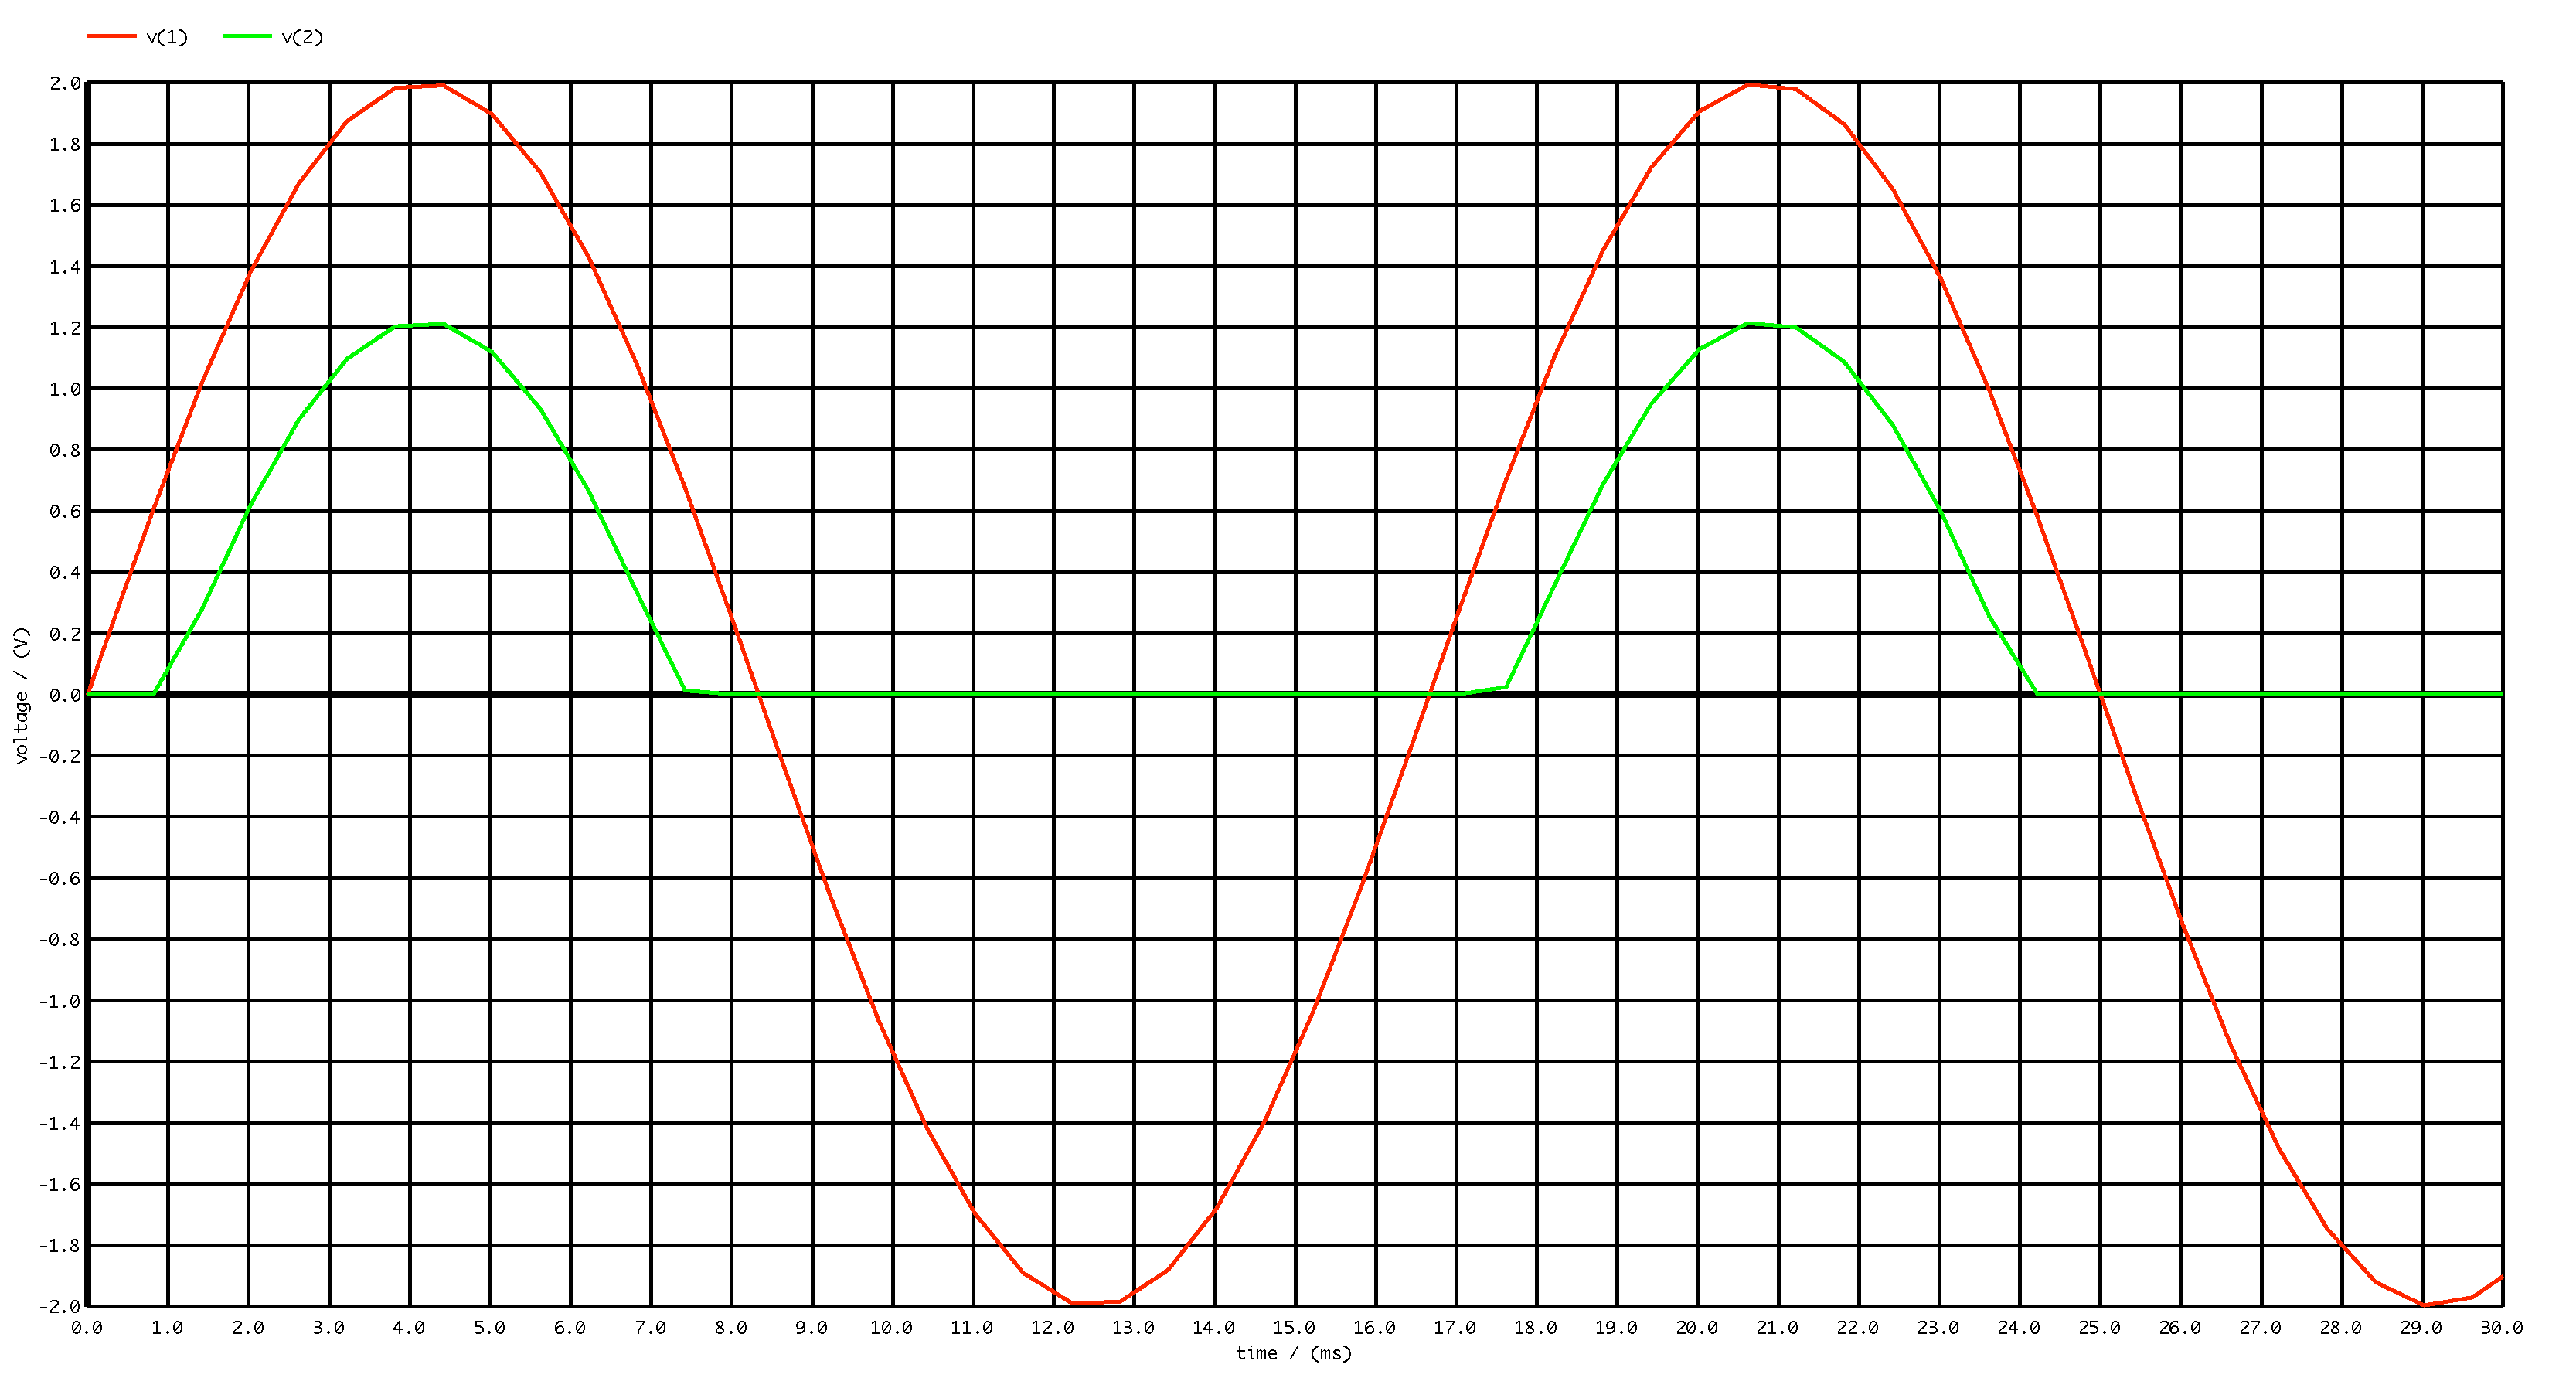
\includegraphics [width=0.8\linewidth]{2_b.pdf}
		\caption{2\_b}
	\end{figure}
\end{enumerate}



\end{document}